\section{introduction}

% meta comment
%The introduction is an overview of the problem; why it is important; a summary of extant work and a statement of your hypothesis or specific question to be explored. Make it readable by anyone. 

% it will be assumed that the target audience is a Physics graduate student. They have not heard of Anderson localization, but they know about wave interference and electrons. No programming experience is assumed, but linear algebra experience is assumed. Multiplication and inverses are known, but self-embedding is not.

% we do not include noise
% -because we are interested in AL/diffusion phenomena
% -experimentally, noise can be supressed

\begin{comment}
% meta comment: what to include generally
-the introduction should not be a comprehensive historical overview [leave that for review articles]. Rather, the reader should be introduced to the minimum historical motivation for the topic. Discuss why the topic is significant, and how this research progresses both the field and society. 
-what advantages does my approach have [why did I chose it instead of other methods]?
\end{comment}

\begin{comment}
introduction shouldn't much contain math. It may have $k \ell \approx 1$, but this will not be derived. It can be cited and explained in words.
\end{comment}

\begin{comment}
the recipie I'm following for my PhD work is
1) simple idea that is usually mathematically intractable [transfer matrix method for long waveguides]
2) new mathematical tool [self-embedding]
3) apply new tool to simple idea [quasi-1D waveguide transport], explain results
\end{comment}

% table: lengths, description, domain of applicability?
% mfp, tmfp, elastic mfp, 
% note: every length can be written as a corresponding time by $length = v_{group} time$.
\begin{center}
\begin{tabular}{ll}
$\lambda_0$ & wavelength of incident light in free space \\ 
$\lambda = \lambda_0/\eta$ & wavelength of light in the medium, refractive index $\eta$ \\ 
$L$ &  system length. Usually normalized by $\lambda_0$ \\ 
$L_D$ & path length. Only defined in ballistic and diffusive regime (Assumes particle definition of light.) \\ 
$\ell_{scat} = \ell_{mfp}$  &  \\ 
$\ell_{tmfp}$ & randomized phase and direction \\ 
$\ell_{tmfp} = \frac{\ell_{scat}}{1-\langle cos \theta \rangle}$ & \\ 
$\ell_{tmfp} \neq \ell_{mfp}$ & \\ 
$\ell_{tmfp} \geqslant \ell_{scat}$ & \\ 
$\xi$ & localization length, probability of loops is 1.  \\ 
$\xi = N \ell_{tmfp}$ &
\end{tabular}
\end{center}


% is this an assumption or fact? Absorption doesn't affect phase

% numerical model collisions are assumed to be elastic (no energy dissapation to heat/excitation)
% numerical model L >> phase coherence length. Valid experimentally for photonic and low temp electronic media

\begin{comment}
% meta comment
For each section:
\begin{itemize}
\item list assumptions
   \begin{itemize}
   \item justify each assumption
   \item why is the assumption needed
   \end{itemize}
\item explain model, based on the assumptions
\item results of the model
\item how results apply to experiment
\end{itemize}
\end{comment}

%Early in the physics education process, we are taught that light can behave as both particles and waves. Which behavior observed is based on the experiment performed. This is because the quantization of light gives it particle-like properties. Matter, on the other hand, is usually thought of as particles, but can behave as waves on a quantum scale. 
%% NOTE: rejected because it doesn't directly contribute to the purpose (which is AL transition). 
For both light and matter, when the particle description is appropriate, transport is quantified by a random walk \glossary{name={random walk}, description={series of uncorrelated choices in direction (and possible step length)}} process called diffusion \cite{2005_Duan_Guojun} \cite{2006_Sheng}. Although waves \glossary{name={wave}, description={undulating electric and magnetic field?}} are present, the average phase and summed interference effects are usually zero. However, when interference due to disorder is dominant, transport is quantified by Anderson Localization. 
%Light propagation is fully described by Maxwell's equations \cite{1999_Jackson}. Any deviation in a theoretical model will need to be explained as to the purpose, and why the system retains the desired phenomena, while not introducing non-physical behavior. 
Although there exists criteria describing the transition between diffusion and Anderson Localization (AL)\index{Anderson Localization}, they apply only in conservative passive media and not directly to active media (where absorption\cite{1998_Brouwer} or gain affects transport) due to lack of conservation. There is currently no criterion describing the transition between diffusion and AL in active random media.
% thesis statement:
The goal of this work is to develop a criterion for the transition to AL from diffusion in active media.% (specifically, with gain). 
This is done by first developing a model of light wave propagation based on Maxwell's equations \cite{1999_Jackson} that can observe AL. 
%Motivation
One application of this criterion would be to determine when lasing in experiments \cite{1999_Cao_RandomLaserPRL} is due to strong localization rather than diffusive random lasing\cite{2008_Wiersma}. Although this work focuses on light, results extend to communities interested in electrical conductance, seismic waves, and astronomy; all needing a description for active rather than passive media. This research is significant as characterization of strong AL of light in three dimensions (3D) has been called the Holy Grail \index{Holy Grail} of optics \cite{1998_POAN}. Although 3D systems are not studied directly in this work, the goal here is to go one step beyond passive media, namely characterizing the transition to AL in active media. 

% outline of chapters:
After an overview of the historical development, current models, and criteria, the physically intuitive models used for this project are developed, starting in one dimension (1D), then planar quasi-one dimensional (quasi-1D). %There exists other models of AL, but the transfer matrix method gives the electric field without Fourier transforms. 

\subsection{Historical outline}
% before discussing various models and criteria, start with definitions of AL, diffusion [concepts]. This is where the history can be put.
Electrical conductivity is described by Ohm's Law $V = I R$ \cite{1917_Millikan}, which is based microscopically on diffusion. Diffusion quantifies a random walk process where electrons scatter from randomly-placed defects in the metal. 
\begin{equation}
 \frac{\partial \psi(\vec{r},t)}{\partial t} = D \nabla^2 \phi(\vec{r},t)
\end{equation}
However, the conductivity was observed to decrease exponentially for various parameter combinations, which was not explained by diffusion. P. W. Anderson, in studying experimentally the metal-insulator transition, was able to describe why conductivity decreased by realizing the importance of electron waves. In the paper entitled ``Absence of diffusion in certain random lattices'' \cite{1958_Anderson}, the deviation from diffusion is explained to be due to wave interference. Wave interference is always present, but is usually not the dominant transport mechanism because the the wave is not coherent long enough to form a closed loop and thus interfere with itself.

For electronic systems, the diffusion equation is an approximation of quantum processes involving matter waves of the electron which breaks down when waves become important. However, the phenomena applies to any wave interaction %in specific circumstances
 where significant random scattering is present. When applying AL to photons, charge conservation is not applicable, and Schrodinger's equation are equivalent to Maxwell equations \cite{1998_POAN}. One way to see the connection between photonic and electronic systems is to state how transmission and conductance are related:
\begin{equation}
 T = \sum_{a,b} |t_{ab}|^2 = g
\end{equation}
where $T$ is the total transmission flux, and $g$ is unitless conductance. With electronic systems, $g$ is what can be measured, whereas in photonic systems, one can also measure
\begin{equation}
\begin{gathered}
 T_a = \sum_b |t_{ab}|^2 \\
 T_{ab} = |t_{ab}|^2
\end{gathered}
\end{equation}
where $T_{ab}$ is speckle. 

% need a strict definition of Diffusion and AL here, so that readers can have something concrete to refer to.
% From andersonlocalization.com,
% In an unbounded localized medium a finite number of bound states per unite volume exists, and the spectrum of the Hamiltonian...becomes dense pointlike. The Hamiltonian has eigenvalues that are infinitely close to each other, and with exponentially localized eigenfunctions. 

Before continuing to the regimes of applicability, current models, and current criteria, diffusion and AL should be defined. This is not a simple discussion and has been contested in liturature since the inception of AL. However, a working definition for passive disordered media is that diffusion is occuring when transmission decreases linearly with system length $L$. Also in passive disordered media, AL is defined as transmission decreasing exponentially with $L$: $T \propto e^{-\frac{L}{\xi}}$, where $\xi$ is the ``localization length.'' For an infinite system, the wave is exponentially localized. In the limit that $L \rightarrow \infty$, both of these phenomena can not be true simultaneously. It turns out that in planar quasi-1D geometry, the diffusing process is characteristic for $L<\xi$, while AL occurs when $L>\xi$. However, since neither diffusion nor AL occurs for all $L$, then one can not claim true AL or diffusion. An experiment or numerical simulation of waves can only claim ``signatures of diffusion'' or ``signatures of AL'' in finite passive media.

When gain or absorption is present in finite media, the experiment or model is then two steps removed from the definition of AL or diffusion. Since an infinite active media either lases (gain) or does not transmit (absorption), then finite active systems must first be re-scaled to passive media, then the finite passive system can be extrapolated to an infinite system to meet AL or diffusion definitions.

So far the physical mechanism, wave interference, and the terms have been defined. Before bringing the reader up to date on current developments, a few key concepts need to be ennumerated about the domains of applicability in order to quantify when AL occurs.

\subsection{transport regimes}
We have already mentioned two possible transport regimes, diffusion  \glossary{name={diffusion}, description={random walk process mathematically describing the flux through a given area}} and Anderson localization\glossary{name={localization}, description={paths long enough to return to same space}}. In both of these, transport is affected by random scatterers. For completeness, a third regime, ballistic\glossary{name={ballistic}, description={very little interaction with scatterers}} transport, occurs when there is very little interaction with scatterers. Each of these regimes are normally defined in (conservative) passive media; that is, no absorption or gain is present. Current criteria for the transition between diffusion and AL apply to passive systems only. These passive regimes can be experimented with by varying the length of the medium for fixed scatterer concentration, or, equivalently, by varying concentration for fixed system length. These two methods are equivalent because they change how much interaction transport has with random scattering. 
% what about aspect ratio (width)?

%As an example to illustrate these regimes, picture shining a light source on a container of milk. If the container is very thin along the direction of light propagation, then light passes through the milk because there is little interaction between light and scatterers (ballistic). As the length of the container of is increased, light diffuses in the milk, and transmission decreases (diffusion).  Alternatively, the length can be fixed and water can be mixed with milk.

There is another set of variations in addition to varying length or concentration: ``active'' media (i.e., absorption or gain \glossary{name={gain}, description={increasing amplitude}}). Experimentally, absorption is normal in everyday materials such as milk (due to phonons or atomic interactions) and the strength of absorption is dependent on material properties. Gain is implemented experimentally by choosing or creating materials with specific atomic characteristics. However, in mesoscopic physics, we disregard the atomic affects in order to model universal behavior. For example, in the 1D numerical model gain is mathematically contrived as an imaginary component of the wave number. This contrivance is acceptable because it yields the desired phenomenon (increasing amplitude coherently as a function of path length) when compared to experiment.

The regimes of ballistic, diffusive, and localized transport have slightly different characteristics depending on the geometry of the medium. The classes of geometries for a given medium are 1D, slab, quasi-1D rectangular, 2D, quasi-1D parallel-piped, and 3D. In this work, we use 1D, slab, quasi-1D rectangular models, and scale the results to higher dimensions \cite{1979_Anderson}. Which geometry applies to a given experiment or numerical simulation is determined by measuring system dimensions $L,W,H$, and the transport mean free path $\ell_{tmfp}$.

%Anderson, in his paper on ``Theory of white paint'' \cite{1985_Anderson}, has a table for passive and absorptive systems. We will add the active portion to that table. 

\subsection{current criteria for passive systems}
Much work has been done in the past 50 years quantifying when transport phenomena transition from diffusion to AL in passive media. As a result, there are multiple definitions for the transition. Although each criteria is not equally useful in a specific experiment, and one can not be derived from another, they are equally valid due to single parameter scaling \cite{1979_Anderson}. 

The first criteria, developed by A. Ioffe and A. Regel \cite{1960_Ioffe_criterion} in 1960, says that when the path length explores more than the area or volume of the waveguide, then loops must form (since the path crosses over itself). Thus the threshold is $ k \ell_{tmfp} \approx 1$ for the AL/diffusion transition. Note that this ``path length'' is an ensemble-averaged quantity. That is, to eliminate behavior specific to a realization\glossary{name={realization}, description={a specific configuration of randomly placed scatterers}}, many realizations are averaged. Averaging (and higher moments of the distribution) are used due to the random nature of the media. Although this Ioffe-Regel criterion is intuitive, it is experimentally difficult to determine the ``path'' of the light and measure when the transition from diffusion to AL occurs. (Note that ray optics are valid only in the diffusive regime, where waves are not expected to play a dominant role.) Thus, there remained motivation to find an easy-to-measure criterion. 

In 1977, Thouless proposed \cite{1977_Thouless} that whether the peaks in density of state were distinguishable or not demonstrated the transition. The ratio of average widths of the density of states (DOS) to peak-to-peak separation returns a unitless number indicating where the experiment is with respect to the transition $\frac{\Delta \omega}{\delta \omega} =1$. %[DOS peaks separated in frequency = localized, peaks overlapping = diffusive]
This was another intuitive criterion, but not always easy to measure in experiment or numerical simulation. 

The transition from diffusion to AL implicitly implies a breakdown of the diffusion process, and by extension, the applicablity of the standard diffusion equation. In an effort to extend the diffusion equation, diagramatic, self-consistant theory \cite{1980_Vollhardt_Wolfle} was developed. Normally, the diffusion coefficient $D_0$ is constant throughout the medium. However, when paths contain loops, the diffusion coefficient decreases. Since loops can not form near the boundary of a sample, the diffusion coefficient becomes position dependent $D(z)$. Thus, the change from constant $D_0$ to position-dependence signifies the transition to AL. 

More recently, A. Genack's \cite{2000_chabanov_nature} correlation fluctuations of conductivity, energy correlation ($\int {\cal E}{\cal E} dz W$), and the inverse participation ratio $\frac{\langle {\cal E}^2 \rangle}{\langle {\cal E} \rangle^2}$ are all measurable and are accepted by the community. New criteria are being suggested, including $\frac{T}{E}$ [cite myself]. However, given all these criteria, making the medium more active than just perturbation of passive media renders each criteria ill-defined. The reason is that each criterion gives in a single numeric value (regardless of the number of input parameters). Varying the length or concentration of random scatterers of a passive medium is a single parameter that yeilds either ballistic, diffusive, or localized regimes. Absorption and gain are two ends of a spectrum that forms a distinct parameter. Thus, any criterion that specifies the location in a two-parameter space must give two numbers (i.e., coordinates in the parameter space). 

Now that we are familiar with the origin of and passive criteria for Anderson Localization, the current numerical models are ennumerated. There are also many experiments for AL, as listed in \cite{2009_Lagendijk_PT}, but these will not be covered in detail here. For example, 1D\cite{2006_Bliokh} and quasi-1D\cite{2008_Genack} microwave metallic waveguides, and ultrasound\cite{2008_van_Tiggelen_Nature}  %http://www.nature.com/nphys/journal/v4/n12/abs/nphys1101.html
\cite{2008_van_Tiggelen}.

\subsection{current transport models}

The standard set of models from solid state , i.e., Bloch waves, Kronig-Penney model, etc. from Chapter 7 of \cite{2005_Kittel}, do not apply because the structure is random instead of periodic. % and more than just perturbation
Since AL depends on wave interference due to random scatterers, analytical treatment is inherently difficult. Thus, numerical modeling is the primary method for exploration of transport phenomena. Computational efforts have so far focused on passive media, where diffusion and AL are defined.

The Anderson tight-binding Hamiltonian \cite{1958_Anderson} uses a random hopping probability for lattice sites. The model has proved useful for scaling predictions for passive media. The downside is assumptions need to be made about the potential, and no visualization of the waveform in the medium is available. Features of the quasi-1D waveguide, such as channels, are not included.

Green's functions can also be used (because?).

For a quasi-1D waveguide, the quantization of transverse modes results in ``channels'' (a set of wave functions determined by boundary conditions).  MacKinnon \cite{2003_Kettemann} gives an overview of transfer matrix and Green's function approachs. Because numerically modeling waveguides using transfer matrices is computationally difficult, in random matrix thoery (RMT)\cite{1951_Wigner} % origin
\cite{1997_Beenakker}, % review, 
the elements of the total transfer matrix are assumed to be random, while obeying certain symmetries (unitarity). 
% get citations from page 103 of Vellekoop's thesis
Then the effect on various parameters is observed when a few more scatterers are added (perturbing the length of the waveguide). As with previous models, RMT does not yield the interior electric field or energy distribution. Also, the incident waveform can not be adjusted. RMT has been very successful at XX.

For this work, the transfer matrix method, introduced by Pendry \cite{1992_Pendry} and extended by MacKinnon, is used. Matching elecric field $E$ and its derivative $E^{\prime}$,
\begin{equation}
 \left( \begin{array}{cc}
T_{11} & T_{12} \\
T_{21} & T_{22} \\
\end{array} \right)
\left( \begin{array}{c}
E_0 \\
E_0^{\prime}
\end{array} \right)
=
\left( \begin{array}{c}
E_{\Delta x} \\
E_{\Delta x}^{\prime}
\end{array} \right)
\end{equation}
where the $\hat{T}$ matrix can be the transition from one layer to another (scatterer or free space), or the product of many layers: $\hat{T} = \Pi \hat{F}\hat{S}$.

The reason the transfer matrix method is difficult is two fold. First, one needs multiple realizations of the disorder to get ensemble-averaged behavior (statistical error is equal to the inverse square root of the number of realizations). The second difficultly is the instability of eigenvalues when numerically multiplying many matrices. These two factors usually limit the method to small systems, i.e. far from the diffusion-AL transition. The advantage to the transfer matrix method is that electric field and energy distribution can be calculated directly (no Fourier tranform necessary). For other models, certain aspects of the system need to be assumed in order to create the model. The transfer matrix method is ab initio, starting from just Maxwell's equations\cite{1999_Jackson}. There are assumptions used, such as scattering potentials, no leakage, conservation of flux.

While many realizations being necessary can be overcome by writing fast and parallel code, the primary impediment to using the transfer matrix method has been numerical eigenvalue instability. One method to deal with this issue is to just use the Lyponov exponent as a measure of localization [explain more]. Another approach is deal with the instability by using Gram-Schmidt orthogonalization of the transfer matrices. The method used here is self-embedding  technique\cite{2001_Yamilov}\cite{1999_yamilov_selfembed}\cite{1976_Bellman_Wing_embedding}. There are multiple basis for the transfer matrix method (outgoing versus incoming flux, left versus right flux) and self-embedding applies to any basis since it applies to any multiplication of matrices.

\subsection{planned research}

Now that the historical origin of AL and what criteria are currently available for passive random media have been covered, we are interested in a criterion for the transition from diffusion to AL in active media. First, a random 1D model is developed. Although 1D systems can inherently not include diffusion, the model gives useful insight to the characteristics of AL. The motivation for 1D is that it is easy to visualize, easily implemented experimentally, and the math is simple. In higher dimensions, as with the quasi-1D model, it will be instructive to retain what was learned in the simpler 1D model. The 1D numerical model is a set of layers of dielectric material \glossary{name={dielectric}, description={index of refraction squared}} where every other layer is of random width. This model is compared to two simpler abstractions; a periodic set of dielectric layers with a single defect, and two potential energy barriers. These two models verify the tunneling effect observed in the random model. The geometry of the 1D numerical model can be specified such that the system is known to be in the localized regime  (and no diffusion is present to confuse results). With this 1D model, we test the usefulness of a new criterion, the ratio of transmission to energy stored in the sample, $T/{\cal E}$. While non-divergent in active media, it is not a single valued function (even in passive media): it depends on the position of the center of localization. Based on this, an improved criterion $\left( \frac{T_g}{E_g}\right)E_p$ is developed. The dependence of the energy distribtion within a specific realization on the center of localization was an unexpected feature. 

After establishing a basic understanding of AL in 1D, the next higher-dimension geometry is a planar quasi-1D metallic waveguide. It is slightly more complicated than 1D, allowing for diffusion and localization. The reason to not go straight to 2D is the mathematically useful quantization of transverse modes, which gives rise to discrete ``channels''\glossary{name={channels}, description={quantized modes of quasi1-1D waveguides}}. Modes of the waveguide can be open or closed, and the first task is to determine the effect of evanescent channels on the  conductance distribution in passive media. Then, in the context of quasi-1D waveguides and multiple transport regimes, a two-parameter space is built (system length versus active media). The goal of the numerical simulations will be to explore this parameter space and verify transitions between transport behaviors.

In passive quasi-1D media, single parameter scaling results in a single parameter space: there exists many possible criterion that can measure whether a given experiment is in the ballistic, diffusive, or localized regime. For example, unitless conductance being greater than unity implies localization, whereas $N_{open}>g>1$ is indicative of diffusion, and $g=N_open$ signifies ballistic transport. Another method is to simply vary system length while maintaining scatterer density. Then sufficiently short systems are ballistic, and sufficiently long systems are localized. The quantification is marked by the scattering length $\ell_{scat}$ and transport mean free path $\ell_{tmfp}$, respectively.

This length basis is used along with a measurement of gain/absorption to construct a two parameter plot. Two parameters are necessary because conservative systems are described by single parameter scaling, and non-conservative media can not be renormalized to passive without overlap. For example, in media with absorption, conductance less than unity does not necessarily imply localization. Conversely for media with gain, conductance greater than unity may still be localized (instead of diffusive). There is an upper limit of two parameters for the space since all media is either conservative or non-conservative. 

In Fig.~\ref{fig:regime_plot_main}, this space is plotted, with length on the horizontal axis and gain on the vertical axis. Gain is chosen as the negative value in accordance with the concept of gain as ``negative absorption'' (although this is not valid due to the existance of a lasing threshold). The horizontal axis can be separated into the three standard regimes: ballistic transport when $L<\ell_{tmfp}$, diffusion for $\ell_{tmfp}<L<\xi$, and localization for $\xi<L$. The space above and below the axis is found to contain distinct ``phases'' of transport behavior. Each phase is denoted by a two letter abbreviation. The A/G refers to absorption/gain, while B/D/G refers to ballistic/diffusive/localized. The regions are seperated by lines determined by the Thouless criterion. In passive media, the Thouless criterion is the ratio of mode width to separation of modes $\delta \omega / \Delta \omega$. In the active media, the mode width is also affected by gain/absorption strength, so the modified Thouless criterion is
\begin{equation}
\frac{\delta \omega +\gamma}{\Delta \omega}
\end{equation}
In Fig.~\ref{fig:regime_plot_main} and Fig.~\ref{fig:regime_lower}, the red line is where the ratio is unity. 

The symmetric $\gamma = \pm \delta \omega$ curves denote where mode width is set by gain/absorption. The intersection of $\gamma = \delta \omega$ and the red $\delta \omega +\gamma=\Delta \omega$ mark a useful point for setting the absorption length. The gain length is symmetrically displaced from the passive axis. 

The horiziontal absorption line extends 

The kink in the curves is the transition from diffusion based equations to Mirlin's projections in the localized regime.

\begin{figure}
\vskip -0.5cm
\centerline{
\scalebox{.75}{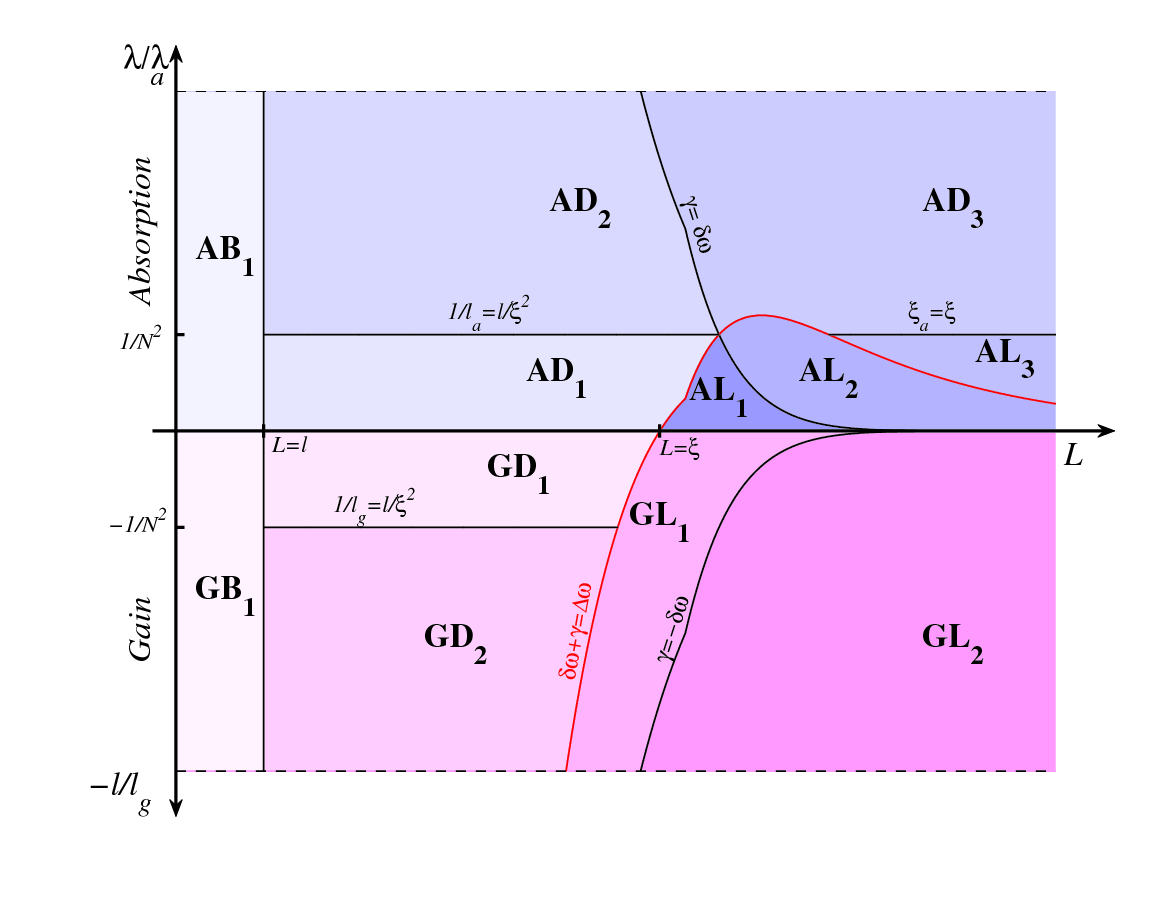
\includegraphics{pictures/regimes_plot_main}}}
\vskip -0.5cm
\caption{Regime plot for quasi-1D random media. Lines denote transitions between regions of similar transport behavior; each region is denoted by a two-letter abbreviation. See text for explanation.}
\label{fig:regime_plot_main}
\end{figure}

The intersection of the curves far from the passive axis are shown separately and are not at the same scale. 

In the very strong absorption regime (c.f. Fig.~\ref{fig:regime_plot_upper})

\begin{figure}
\vskip -0.5cm
\centerline{
\scalebox{.75}{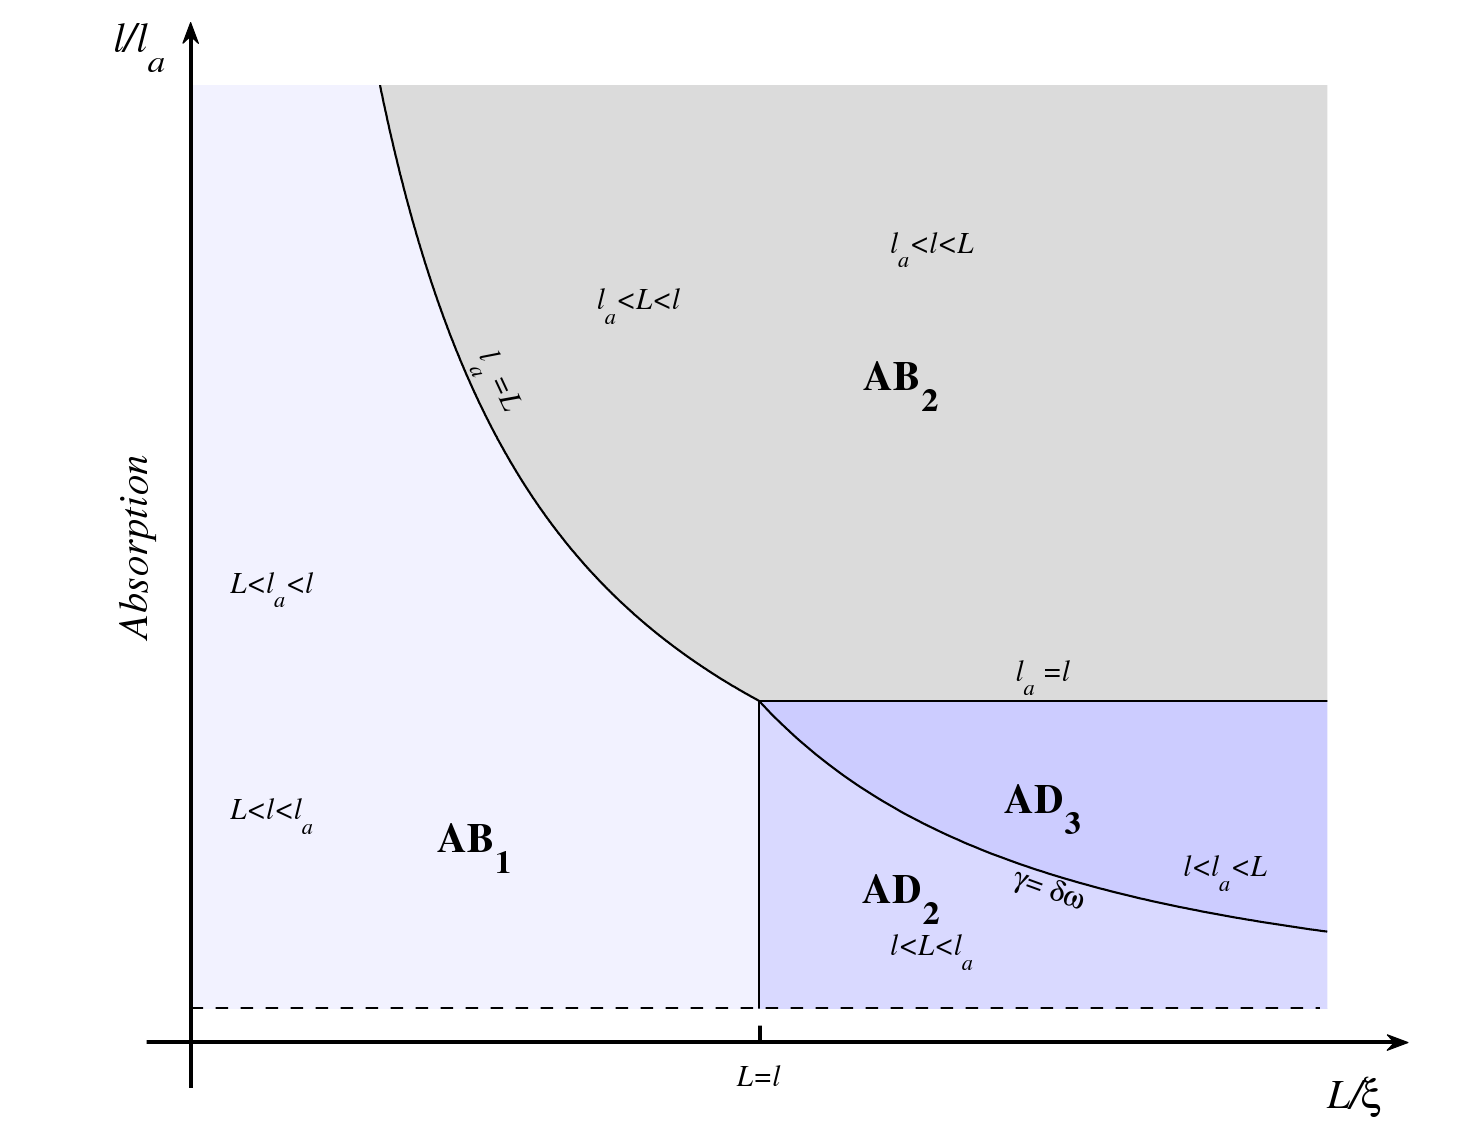
\includegraphics{pictures/regimes_plot_upper}}}
\vskip -0.5cm
\caption{Upper regime plot (strong absorption) for quasi-1D random media. Each region is associated with an inequality of lengths. See text for explanation.}
\label{fig:regime_plot_upper}
\end{figure}

When sufficent gain leads to lasing (c.f. Fig.~\ref{fig:regime_plot_lower}), there are four different reasons the lasing occurs. If the gain length is less than the system length (blue curve $\ell_g =L$), ballistic lasing is expected for the majority of random media. 

\begin{figure}
\vskip -0.5cm
\centerline{
\scalebox{.75}{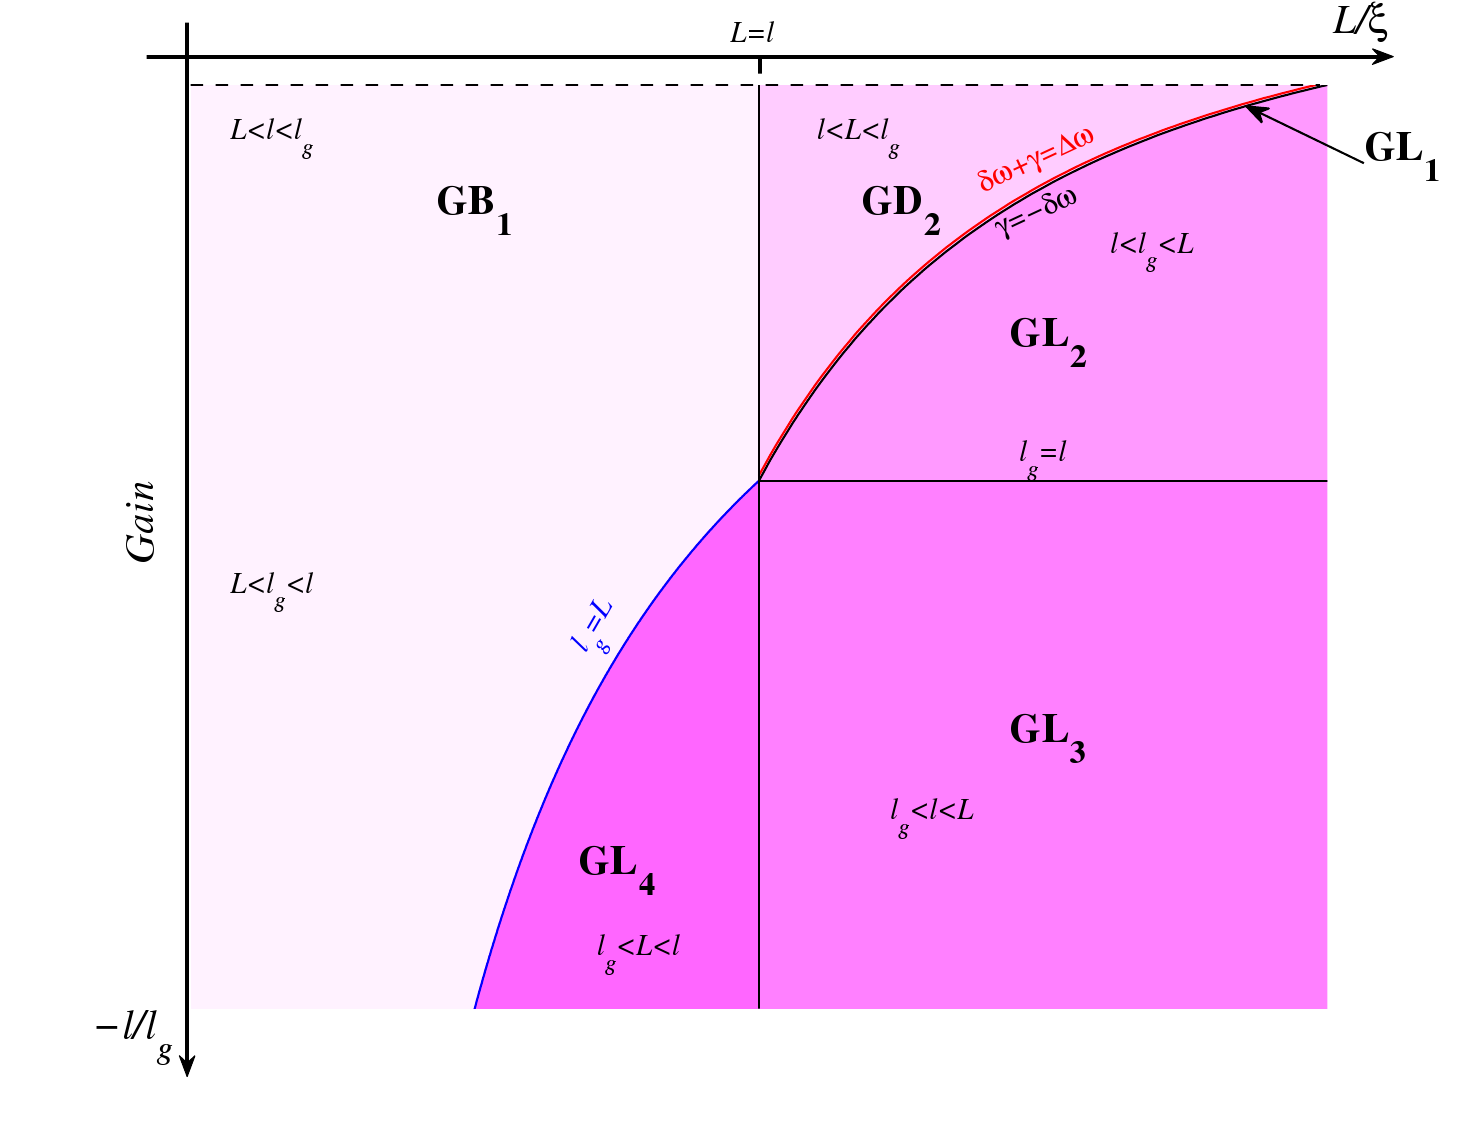
\includegraphics{pictures/regimes_plot_lower}}}
\vskip -0.5cm
\caption{Lower regime plot (strong gain) for quasi-1D random media. See text for explanation.}
\label{fig:regime_plot_lower}
\end{figure}

Using the quasi-1D numerical model described in XX, the two parameter phase space described above will be investigated. While simulating a statistically significant number of realizations ($10^6$), the criteria listed above are recorded. Altough the criteria only work for passive systems, it will be useful to understand how each criterion behaves in non-convservative random media in ballsitic, diffusive, and localized regimes. Specifically, the criteria found are
\begin{itemize}
\item The ratio of transmission to energy stored in the medium $T/{\cal E}$, $\left(T_g/{\cal E}_g\right){\cal E}_p$, and associated channel resolved versions. The values for each $T$ and ${\cal E}$ are initially recorded, then respective ratios are analyzed in post-processing\glossary{name={post-processing}, description={analysis carried out after and separate from the initial numerical simulation. In this case, usually refers to matlab script analyzing Fortran 90 results.}}
\item position dependent diffusion coefficient $D(z)$ from self-consistent theory of localization \cite{2008_Cherroret}, constructed in post-processing from energy density and interior flux
\item energy correlation 
\item conductance $g$
\item eigenvalues of transmission
\end{itemize}
Each of these criteria alone are not expected to be able to accurately describe the localization-diffusion transition in non-conservative media. However, the behavior of each should change at the phase boundaries in Fig.~\ref{fig:regime_plot_lower}\ref{fig:regime_plot_upper}\ref{fig:regime_plot_main}

\begin{comment}
\subsection{jargon definitions}
terms to define (a checklist)
\begin{itemize}
%\glossary{name={}, description={}}
\item laser \glossary{name={laser}, description={light amplification stimulated emission radiation}}
\item elastic collision \glossary{name={elastic collision}, description={kinetic energy is same after event as before}}
\item inelastic collision \glossary{name={inelastic collision}, description={kinetic energy not conserved (heat, excitation}}
\item random versus disordered: interchangeable? \\
The scatterers in a medium should be randomly placed. For 1D slabs, the width of a ``random'' slab is uniformly distributed $1 \pm 0.2$. In our quasi-1D models, random placement of scatterers is complicated by the caveat that if two scatterers are too close, then closed channels dominate transport. By placing a lower bound on separation, a finite number of closed channels adequately describe transport.
\item electron \glossary{name={electron}, description={}}
\item amplitude \glossary{name={amplitude}, description={height of wave function}} can be negative or positive, whereas magnitude $\equiv |\text{amplitude}|$
\item intensity \glossary{name={intensity}, description={}}
\item flux \glossary{name={flux}, description={$\Phi = |Amplitude|^2 k k_{\parallel}$}}
\item transmission \glossary{name={transmission}, description={}}
\item reflection \glossary{name={reflection}, description={}}
\item Fresnel equations \\
http://scienceworld.wolfram.com/physics/FresnelEquations.html \\
$T = |t|^2$ and $R = |r|^2$. Upper case denotes power, aka intensity; lower case for field amplitude coefficient
\item transmittance \glossary{name={transmittance}, description={the ratio of transmission to incident intensity, and it is thus unit-less. Sometimes expressed as a percentage http://scienceworld.wolfram.com/physics/Transmittance.html }} 
\item reflectance \glossary{name={reflectance}, description={}}
\item absorbance \glossary{name={absorbance}, description={}} 
http://scienceworld.wolfram.com/physics/Absorbance.html \\
http://en.wikipedia.org/wiki/Transmittance\\
$A \equiv -log(T)$ \\
\item Beer-Lambert law [empirical]: $dI = -I \rho dl$. See also transmittance, absorbance \\
http://en.wikipedia.org/wiki/Beer-Lambert\_law
\item diffuson, cooperon
\item complex number \glossary{name={complex number}, description={linear combination of real (a) and complex number (b) in the form $a+ib$.}}
\end{itemize}
\end{comment}